% Meine Packages und Optionen
\documentclass[draft=false
              ,paper=a4
              ,twoside=false
              ,fontsize=10pt
              ,headsepline
              ,BCOR10mm
              ,DIV10
              ]{scrbook}

\usepackage[left=2cm,right=2cm,top=1cm,bottom=1cm,includeheadfoot]{geometry}              
\usepackage[ngerman]{babel}
\usepackage[T1]{fontenc}
\usepackage[utf8]{inputenc}
\usepackage[german,refpage]{nomencl}
\usepackage[pdftex]{graphicx}
\usepackage[usenames,dvipsnames,svgnames,table]{xcolor}
\usepackage[automark,autooneside]{scrpage2}
\usepackage{xkeyval}
\usepackage{calc}
\usepackage[absolute]{textpos}
\usepackage{lipsum}
\usepackage[table]{xcolor} % Für farbige Tabellenzellen
\usepackage{colortbl} % Für farbige Tabellenzellen mit cellcolor
\usepackage{listings}
\usepackage{caption}
\DeclareCaptionFont{white}{\color{white}}
\DeclareCaptionFormat{listing}{%
  \parbox{\textwidth}{\colorbox{gray}{\parbox{\textwidth}{#1#2#3}}\vskip-4pt}}
\captionsetup[lstlisting]{format=listing,labelfont=white,textfont=white}
\lstset{frame=lrb,xleftmargin=\fboxsep,xrightmargin=-\fboxsep}
\renewcommand\lstlistingname{Konsolenausgabe} % Listing Name

\begin{document}
\selectlanguage{ngerman}
%Source für das Titelblatt
%\title{Titel des Dokumentes}
%\author{Max Muster}
%\date{01.01.0001}
%\maketitle
\begin{titlepage}


 \def\theThesisAuthor{Mario Hanna, Matthias Szykora}
 \def\theThesisType{Praktikumsprotokoll}
 \def\theThesisTitle{Versuch 2: Statisches Routing}
 \def\theThesisSubTitle{Rechnernetze}
 
  \thispagestyle{empty}%
  \enlargethispage{\footskip}%
  \setlength{\parindent}{0em} % remove indent
  \sffamily % the title page in sans serif

  \begin{textblock*}{2cm}(10cm,2cm)
    \begin{minipage}[r]{\textwidth}%
      \if@haw@printer % hide logo if printer is true
      \relax
      \else
      
\includegraphics[width=10cm]{pic/logo}%
      \fi
    \end{minipage}%
  \end{textblock*}

  %% color bar
  \begin{textblock*}{11cm}(0cm,9cm)
    \colorbox{SkyBlue}{%
      %% use a minipage that is the size of the colored banner
      %% center the minipage
      \begin{minipage}[l][10cm][c]{\paperwidth}%
        %% put the box on the right side
        \hspace*{0.25\textwidth}
        \parbox[t]{0.7\textwidth}{%
          {\centering\bfseries\Huge\theThesisType

          \bigskip
          \Large\theThesisAuthor

          \vspace{2em}
          \theThesisTitle

          \bigskip
          \large\theThesisSubTitle\par
        }}%
      \end{minipage}%
    }
  \end{textblock*}



  \newlength{\xpos}
  \newlength{\fw}
  \setlength{\xpos}{1.5cm}
  \setlength{\fw}{\paperwidth}
  \addtolength{\fw}{-12\xpos}
  
  \begin{textblock*}{2cm}(\xpos,0.85\paperheight)
    \begin{minipage}[c]{\fw}
      \centering\newlength{\tw}
      \settowidth{\tw}{Studiendepartment Informations- und Elektrotechnik}
      \parbox[t]{\tw}{%
        \normalfont\itshape%
        Fakultät Technik und Informatik\\
        Technische Informatik
      }
    \end{minipage}
  \end{textblock*}

\null
\newpage

\end{titlepage}

%Inhaltsverzeichnis
\tableofcontents
       
\newpage
\chapter{Aufgabenteil 1 - Netzwerke untersuchen}
Zunächst soll im Rahmen der Aufgabe die Kommunikation zwischen zwei bestimmten Rechnern in verschiedenen Netzen über statisches Routing realisiert werden. Von uns benutzte Rechner waren LAB28 (Arbeitsrechner) und LAB37 (Gegenstellenrechner).
\newline
\newline
\textbf{LAB28} besitzt die IP-Adresse 192.168.18.132 am Netzwerkinterface eth1 und hatte folgende statische Routen konfiguriert.

\begin{lstlisting}[label=lab28,caption=LAB28]
networker@lab28:~> sudo /sbin/route -n
Kernel IP routing table
Destination     Gateway         Genmask         Flags Metric Ref    Use Iface
0.0.0.0         141.22.26.1     0.0.0.0         UG    0      0        0 eth0
141.22.26.0     0.0.0.0         255.255.254.0   U     0      0        0 eth0
172.16.1.0      0.0.0.0         255.255.255.0   U     0      0        0 eth2
192.168.18.0    0.0.0.0         255.255.255.0   U     0      0        0 eth1
\end{lstlisting}
\textbf{LAB37} besitzt die IP-Adresse 192.168.17.17 am Netzwerkinterface eth1 und hatte folgende statische Routen konfiguriert.

\begin{lstlisting}[label=lab37,caption=LAB37]
networker@lab37:~> /sbin/route -n
Kernel IP routing table
Destination     Gateway         Genmask         Flags Metric Ref    Use Iface
0.0.0.0         141.22.26.1     0.0.0.0         UG    0      0        0 eth0
141.22.26.0     0.0.0.0         255.255.254.0   U     0      0        0 eth0
172.16.1.0      0.0.0.0         255.255.255.0   U     0      0        0 eth2
192.168.17.0    0.0.0.0         255.255.255.0   U     0      0        0 eth1
\end{lstlisting}
In den beiden obigen Listings sieht man, dass sich die Rechner nicht über ihre Routen erreichen können, da beide Rechner keine Route ins jeweils andere Netz kennen.
\section{Paketvermittlung über den Knotenrechner}
\subsection{ARP und Routingtabelle}
Damit eine Verbindung zwischen den Netzen möglich wird, werden die Routingtabellen der Rechner LAB28 und LAB37 entsprechend konfiguriert.
Über das Gateway 192.168.18.2 (RNS1) wird die Route auf LAB28 ins Netz 192.168.17.0/24 ermöglicht.

\begin{lstlisting}[label=lab28knoten,caption=Konfigurierte Route ins Netz 192.168.17.0/24 auf LAB28]
networker@lab28:~> sudo /sbin/route add -net 192.168.17.0/24 gw 192.168.18.2 eth1
networker@lab28:~> /sbin/route -n
Kernel IP routing table
Destination     Gateway         Genmask         Flags Metric Ref    Use Iface
0.0.0.0         141.22.26.1     0.0.0.0         UG    0      0        0 eth0
141.22.26.0     0.0.0.0         255.255.254.0   U     0      0        0 eth0
172.16.1.0      0.0.0.0         255.255.255.0   U     0      0        0 eth2
192.168.17.0    192.168.18.2    255.255.255.0   UG    0      0        0 eth1
192.168.18.0    0.0.0.0         255.255.255.0   U     0      0        0 eth1 
\end{lstlisting}
Die Route für LAB37 ins Netz 192.168.18.0/24 wird über das Gateway 192.168.17.2 (RNS1) realisiert.

\begin{lstlisting}[label=lab37knoten,caption=Konfigurierte Route ins Netz 192.168.18.0/24 auf LAB37]
networker@lab37:~> sudo /sbin/route add -net 192.168.18.0/24 gw 192.168.17.2 eth1
networker@lab37:~> /sbin/route -n
Kernel IP routing table
Destination     Gateway         Genmask         Flags Metric Ref    Use Iface
0.0.0.0         141.22.26.1     0.0.0.0         UG    0      0        0 eth0
141.22.26.0     0.0.0.0         255.255.254.0   U     0      0        0 eth0
172.16.1.0      0.0.0.0         255.255.255.0   U     0      0        0 eth2
192.168.17.0    0.0.0.0         255.255.255.0   U     0      0        0 eth1
192.168.18.0    192.168.17.2    255.255.255.0   UG    0      0        0 eth1
\end{lstlisting}
Sendet man nun eine Anfrage von LAB28, zu einem beliebigen Rechner im Netz 192.168.17.0/24, muss, sofern nicht bereits in der ARP-Tabelle vorhanden, zunächst die MAC-Adresse des Gateways ermittelt werden, damit die Anfragen von dort aus weitervermittelt werden können. In Konsolenausgabe 1.5 sieht man die ARP-Tabelle inkl. der MAC-Adresse zur IP 192.168.18.2 .

\begin{lstlisting}[label=arbknoten,caption=ARP Request und Replay zwischen RNS1 und LAB28]
networker@lab28:~> /sbin/arp
Address                  HWtype  HWaddress           Flags Mask            Iface
141.22.26.1              ether   6c:50:4d:ae:b4:00   C                     eth0
192.168.18.2             ether   a0:36:9f:16:cb:a9   C                     eth1
networker@lab28:~> 
\end{lstlisting}
\subsection{Paketwege}
Mit Traceroute und der Record Route Option (ping-R) wurde die Wegewahl beim Routing ermittelt.
\subsubsection{Traceroute}
Bei der Traceroute wird zunächst, ein IP Paket mit TTL = 1 verschickt. Dieses Paket wird am nächsten Netzknoten, der die Pakete auf dem IP-Layer betrachtet um 1 verringert. Ist der TTL- Wert bei 0, wird das IP-Paket verworfen und an den Absender eine ICMP- Nachricht (Time-To-Live Exceeded) geschickt. Anhand der Absenderadresse des ICMP-Packets kann Traceroute ermitteln wie weit die Anfrage gekommen ist. Jetzt kann ein Packet mit TTL = 2 losgeschickt werden, um den nächsten Hop zu ermitteln. Dieses Verfahren wird solange betrieben, bis man entweder am gesuchten Ziel ist (ICMP-Meldung: Port unreachable) oder ein maximaler TTL Wert überschritten wurde. Ansonsten ist noch zu erwähnen das die Anfragen das verbindungslose Protokoll UDP als Transportprotokoll verwenden.
\begin{lstlisting}[label=traceknoten,caption=Traceroute Ausgabe]
networker@lab28:~> /usr/sbin/traceroute 192.168.17.17
traceroute to 192.168.17.17 (192.168.17.17), 30 hops max, 60 byte packets
 1  192.168.18.2 (192.168.18.2)  0.172 ms  0.161 ms  0.157 ms
 2  192.168.17.17 (192.168.17.17)  0.410 ms  0.406 ms  0.493 ms
networker@lab28:~>
\end{lstlisting}
In Konsolenausgabe 1.6 sieht man die Ausgabe von Traceroute. Es lässt sich erkennen, dass LAB37 über einen Hop (RNS1) von LAB28 erreichbar ist. Zudem erkennt man in der unteren Abbildung 1.1 den gesnifften Kommunikationsverlauf welchen Traceroute ausgelöst hat.

\begin{figure}[htb]
	\centering
  	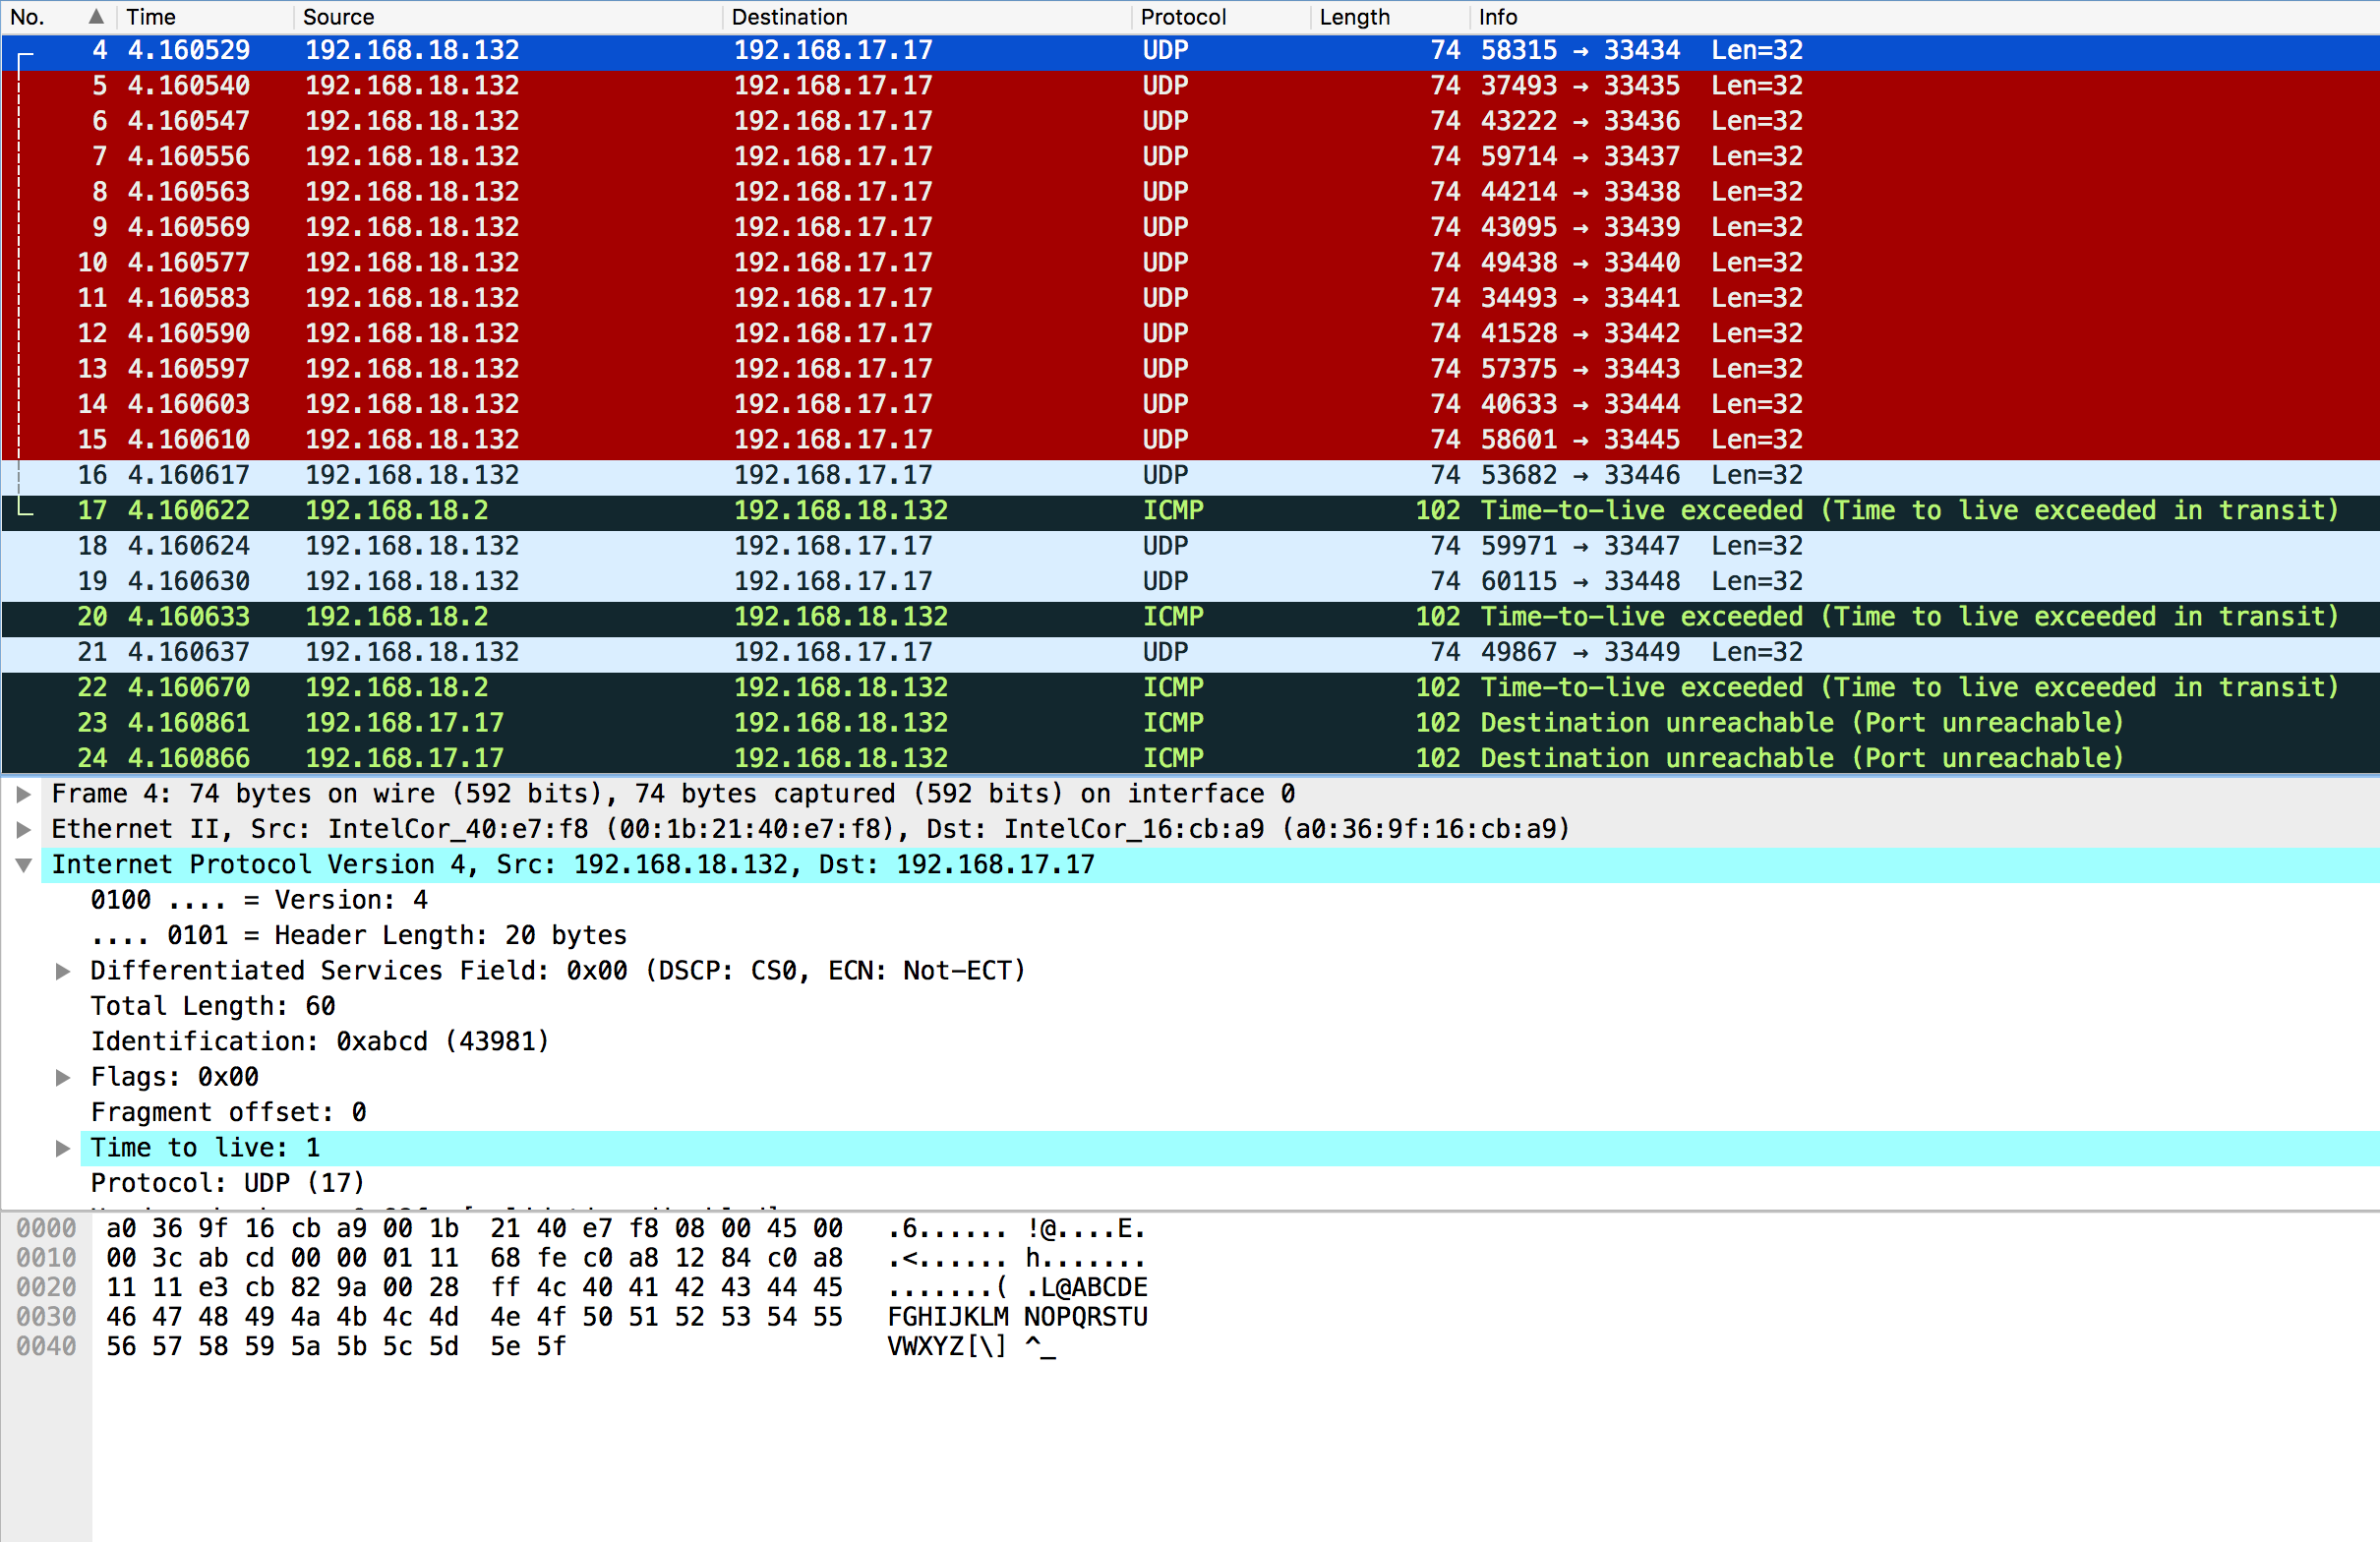
\includegraphics[scale = 0.27]{pic/tracerouteKnoten}	
  	\caption{Wireshark - Traceroute}
	\label{fig1}
\end{figure}
\newpage
\subsubsection{Record Route Option (ping-R)}
Im Befehl Ping setzt die -R Option die Record Route Option in den Echo-Request Paketen, welche gesendet werden. Dadurch können bis zu neun Router an denen der Echo-Request und der folgende Echo-Replay vorbeikommen, ihre IP-Adresse eintragen. So kann die Route beim Empfänger ausgelesen werden. 
\newline
\newline
\begin{figure}[htb]
	\centering
  	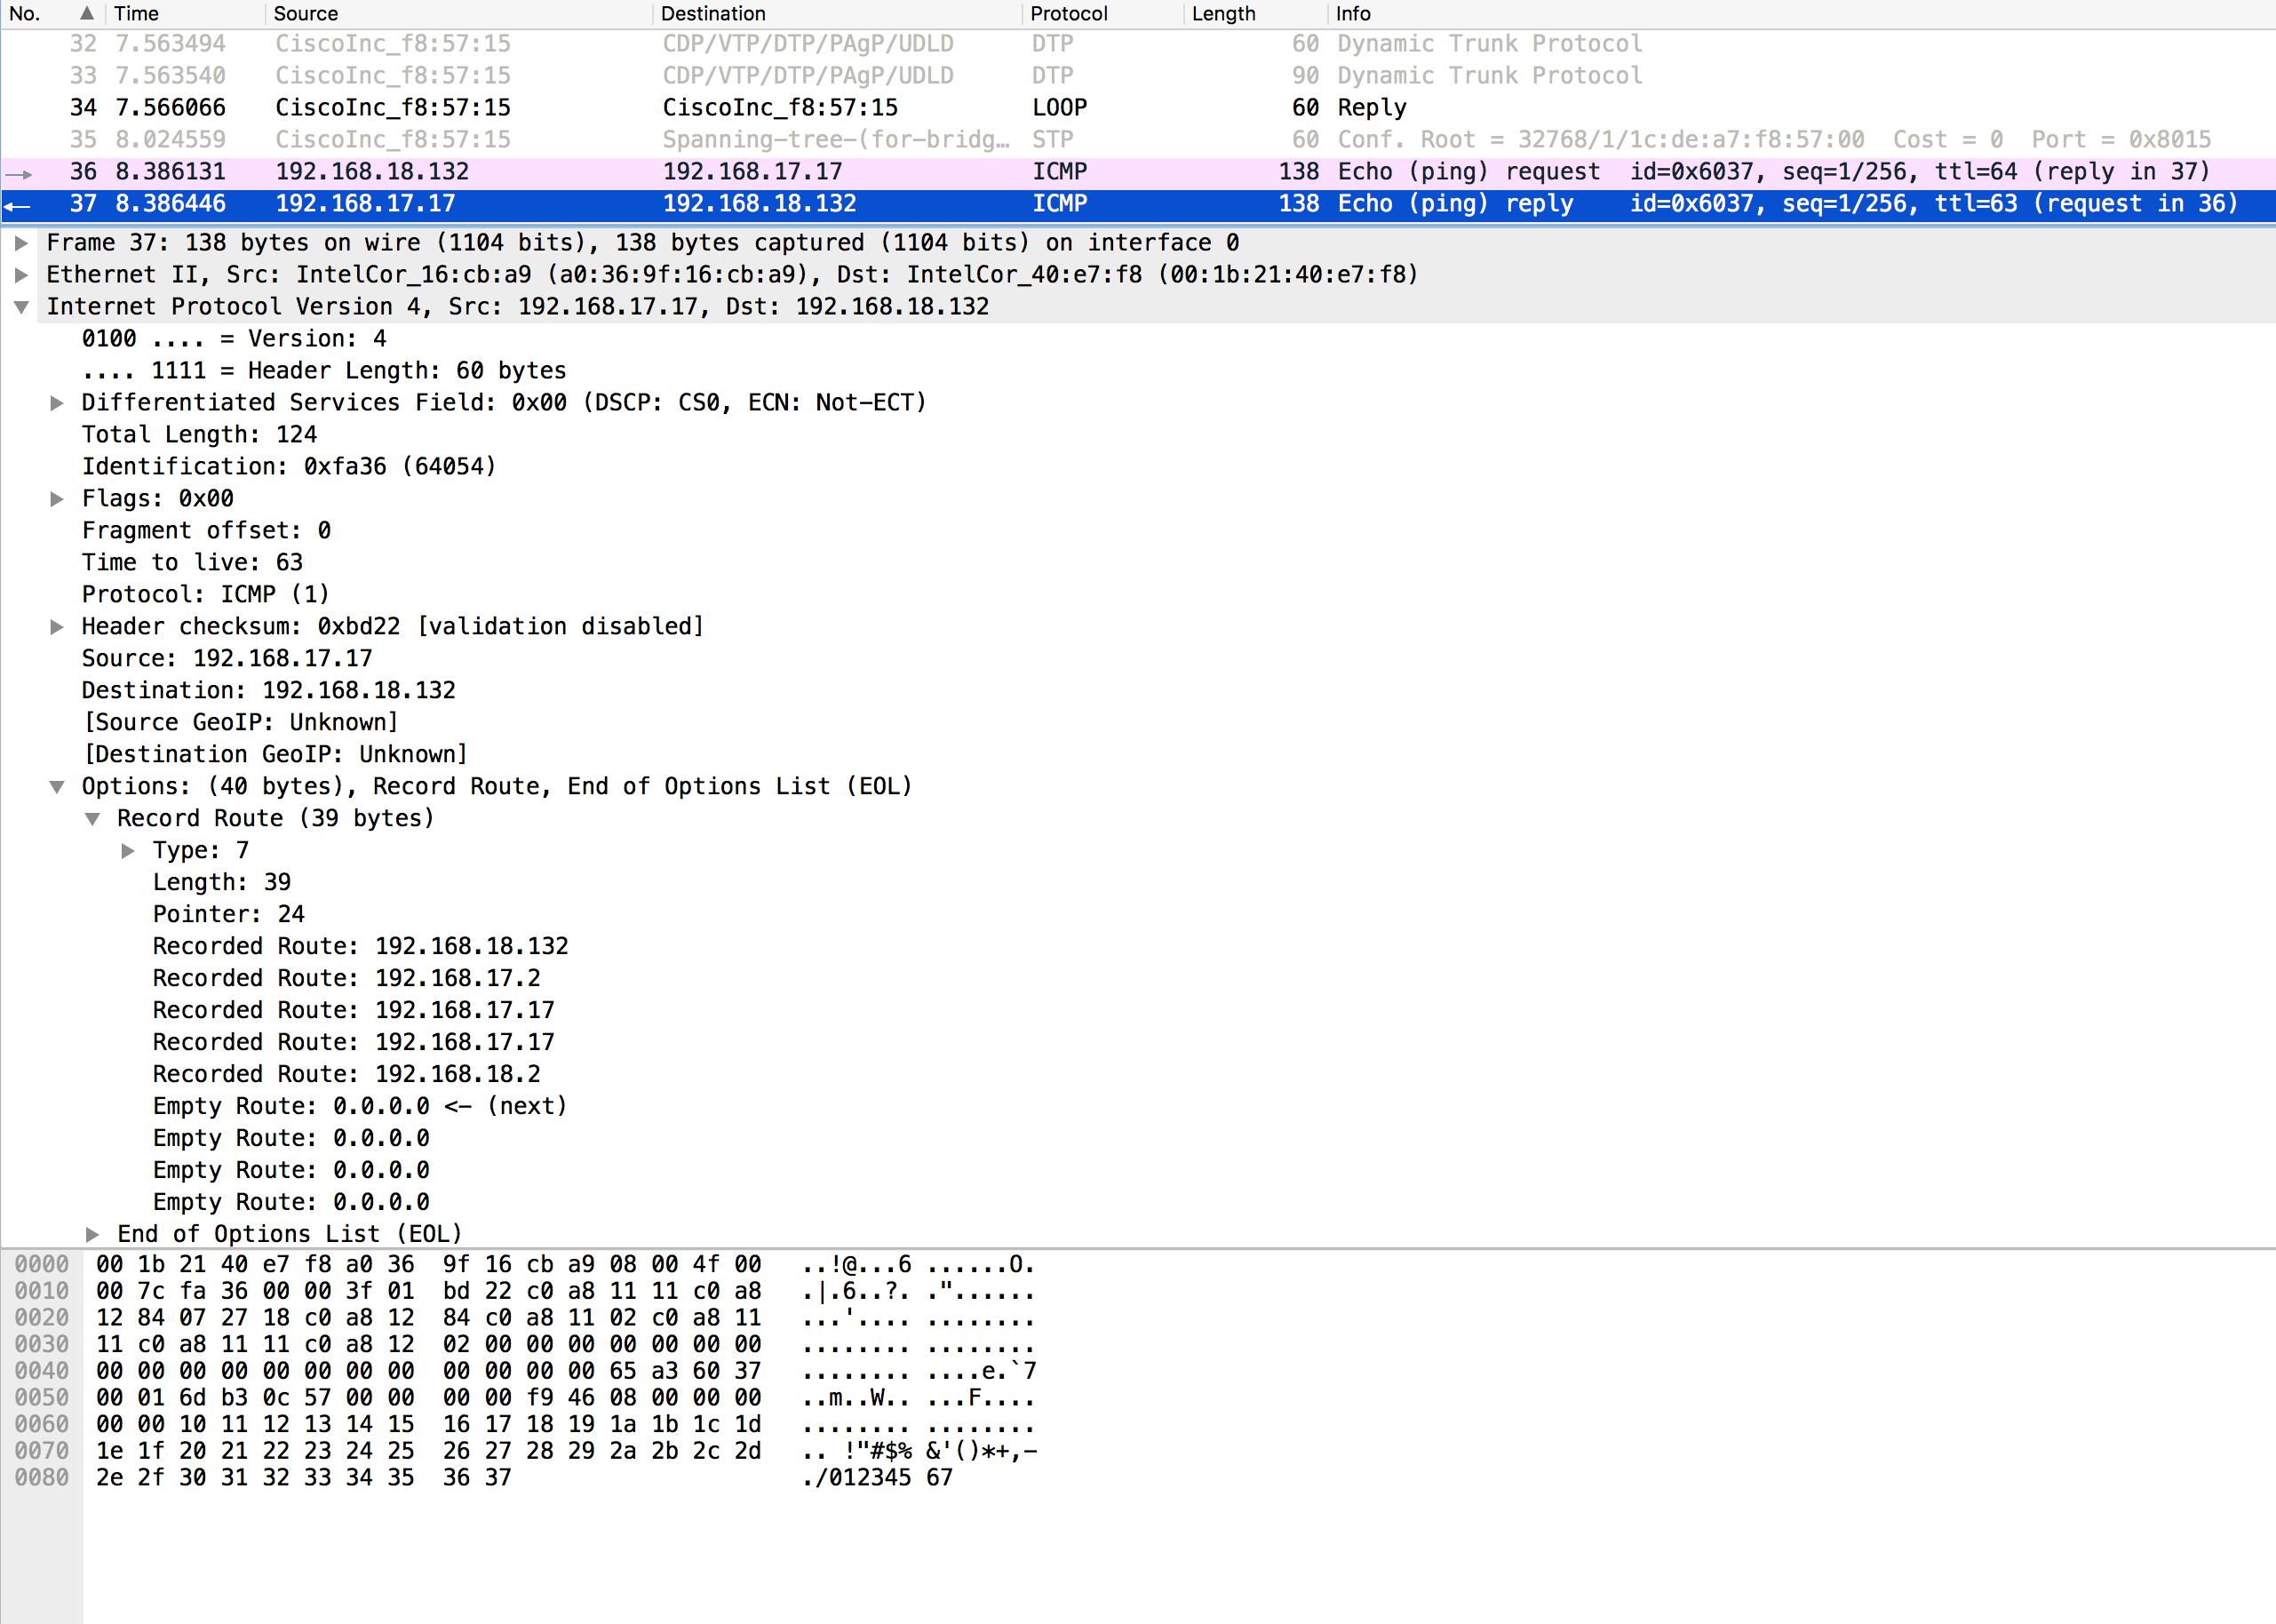
\includegraphics[scale = 0.27]{pic/pingRKnoten}
  	\caption{Whireshark - ping -R}
	\label{fig2}
\end{figure}

\newpage
\begin{lstlisting}[label=pingRknoten,caption=ping -R Konsolenausgabe]
networker@lab28:~> ping -R 192.168.17.17
PING 192.168.17.17 (192.168.17.17) 56(124) bytes of data.
64 bytes from 192.168.17.17: icmp_seq=1 ttl=63 time=0.350 ms
RR:     192.168.18.132
        192.168.17.2
        192.168.17.17
        192.168.17.17
        192.168.18.2
        192.168.18.132

64 bytes from 192.168.17.17: icmp_seq=2 ttl=63 time=0.351 ms    (same route)
64 bytes from 192.168.17.17: icmp_seq=3 ttl=63 time=0.334 ms    (same route)
64 bytes from 192.168.17.17: icmp_seq=4 ttl=63 time=0.298 ms    (same route)
\end{lstlisting}
\subsection{Datendurchsatz}
Der Datendurchsatz wird mit dem Befehl netperf gemessen. Ein Server-Programm (netserver) auf dem Zielrechner (LAB37) rechnet die Datenmenge und die Zeit, in der Pakete gesendet bzw. empfangen werden, und misst daraus den Performance-Wert.
\begin{lstlisting}[label=netperfknoten,caption=Datendurchsatz]
networker@lab28:~> /usr/local/netperf/netperf -H 192.168.17.17
TCP STREAM TEST to 192.168.17.17
Recv	Send	Send	
Socket	Send	Message	Elapsed
Size	Size	Size	time	Throughput
bytes 	bytes	bytes	secs.	10^6bits/sec

 87380	 16384	16384	10.00	 759.02
networker@lab28:~>
\end{lstlisting}

\newpage
\section{Paketvermittlung über die ISDN-Strecke}
Um die Routen der ISDN-Strecke zu betrachten werden die Routen über RNS1 gelöscht.
\subsection{ARP und Routingtabelle}
Im wesentlichen ist das Vorgehen beim Einrichten der Routen Identisch mit dem vorherigen Aufgabenteil. Der einzige Unterschied liegt in der Wahl der Gateways für die Vermittlung zwischen den Netzen.
\begin{lstlisting}[label=arbeitsRechnerISDN,caption=Konfigurierte Routen auf LAB28]
networker@lab28:~> sudo /sbin/route add -net 192.168.17.0/24 gw 192.168.18.1 eth1
networker@lab28:~> /sbin/route -n
Kernel IP routing table
Destination     Gateway         Genmask         Flags Metric Ref    Use Iface
0.0.0.0         141.22.26.1     0.0.0.0         UG    0      0        0 eth0
141.22.26.0     0.0.0.0         255.255.254.0   U     0      0        0 eth0
172.16.1.0      0.0.0.0         255.255.255.0   U     0      0        0 eth2
192.168.17.0    192.168.18.1    255.255.255.0   UG    0      0        0 eth1
192.168.18.0    0.0.0.0         255.255.255.0   U     0      0        0 eth1
\end{lstlisting}

\begin{lstlisting}[label=gegenStelleISDN,caption=Konfigurierte Routen auf LAB37]
networker@lab37:~> sudo /sbin/route add -net 192.168.18.0/24 gw 192.168.17.1 eth1
networker@lab37:~> /sbin/route -n
Kernel IP routing table
Destination     Gateway         Genmask         Flags Metric Ref    Use Iface
0.0.0.0         141.22.26.1     0.0.0.0         UG    0      0        0 eth0
141.22.26.0     0.0.0.0         255.255.254.0   U     0      0        0 eth0
172.16.1.0      0.0.0.0         255.255.255.0   U     0      0        0 eth2
192.168.17.0    0.0.0.0         255.255.255.0   U     0      0        0 eth1
192.168.18.0    192.168.17.1    255.255.255.0   UG    0      0        0 eth1
\end{lstlisting}
Auch hier wird durch einen Ping-Befehl zu einen Rechner im Netz 192.168.17.0/24 von LAB28 aus, zunächst per ARP die MAC-Adresse des zugeordneten Gateways erfragt. 
\begin{lstlisting}[label=arbISDN,caption=ARP auf LAB28 nach ping auf 192.168.17.17]
networker@lab28:~> /sbin/arp
Address                  HWtype  HWaddress           Flags Mask            Iface
141.22.26.1              ether   6c:50:4d:ae:b4:00   C                     eth0
192.168.18.1             ether   00:60:47:50:39:44   C                     eth1
networker@lab28:~> 
\end{lstlisting}
\subsection{Paketwege}
\subsubsection{Traceroute}
Die Konsolenausgabe für Traceroute zeigt, dass ein Teil der Kommunikation nicht ermittelt werden konnte.
\begin{lstlisting}[label=tracerouteISDN,caption=ISDN-Strecke traceroute]
networker@lab28:~> /usr/sbin/traceroute 192.168.17.17
traceroute to 192.168.17.17 (192.168.17.17), 30 hops max, 60 byte packets
 1  192.168.18.1 (192.168.18.1)  4.483 ms  6.014 ms  7.558 ms
 3  * * *
 2  192.168.17.17 (192.168.17.17)  68.942 ms  80.098 ms  92.523 ms
networker@lab28:~>
\end{lstlisting}
\subsubsection{Record Route Option (ping-R)}
Im Vergleich zu Traceroute erkennt ping -R Hin und Rückwege ohne Probleme. Zudem sind erwartungsgemäß die Antwortzeiten um ein Vielfaches höher als die gemessen Zeiten in der vorherigen Versuchsphase.
\begin{lstlisting}[label=pingRISDN,caption=ISDN-Strecke ping -R 192.168.17.17]
networker@lab28:~> ping -R 192.168.17.17
PING 192.168.17.17 (192.168.17.17) 56(124) bytes of data.
64 bytes from 192.168.17.17: icmp_seq=1 ttl=62 time=48.5 ms
RR:     192.168.18.132
	192.168.20.2
	192.168.17.1
        192.168.17.17
        192.168.17.17
        192.168.20.1
        192.168.18.1
        192.168.18.132

64 bytes from 192.168.17.17: icmp_seq=2 ttl=62 time=48.4 ms    (same route)
64 bytes from 192.168.17.17: icmp_seq=3 ttl=62 time=48.4 ms    (same route)
64 bytes from 192.168.17.17: icmp_seq=4 ttl=62 time=48.5 ms    (same route) 
\end{lstlisting}
\subsection{Datendurchsatz}
Auch hier wurde der Datendurchsatz der ISDN-Strecke mit den Tools netperf und netserver gemessen.
\begin{lstlisting}[label=netperfISDN,caption=ISDN-Strecke Datendurchsatz]
networker@lab28:~> /usr/local/netperf/netperf -H 192.168.17.17
TCP STREAM TEST to 192.168.17.17
Recv	Send	Send	
Socket	Send	Message	Elapsed
Size	Size	Size	time	Throughput
bytes 	bytes	bytes	secs.	10^6bits/sec

 87380	 16384	16384	21.99	   0.05
networker@lab28:~>
\end{lstlisting}
In Konsolenausgabe lässt sich erkennen, dass Datendurchsatz viel geringer ist als in der vorherigen Messung.
\section{Fazit}
\subsection{Traceroute - Record Route Option (ping -R)}
Record Route Option (ping -R), als im ICMP nativ vorgesehenes Diagnosetool, hat den großen Vorteil, dass es Rückwege erfassen. Aufgrund der Beschränkung auf neun trackbare Hops ist es zur Diagnose über viele Netze hinweg kaum geeignet.
\newline
Bei Traceroute ist der Vorteil, dass es Vermittlungspfade über nahezu beliebig lange Routen ermitteln kann.
Jedoch erkennt Traceroute keine Rückwege und es nicht gewährleistet, dass alle Routingknoten korrekt erkannt werden.
\subsection{Datendurchsatz RSN1 - ISDN-Strecke}
Vergleicht man die beiden Messergebnisse zeigt sich, dass die ISDN Verbindung eine deutlich kleinere Bandbreite besitzt, als die der Router RNS1.
Laut Messung wurden beim Routing über RNS1 759.02 MBit/s gemessen. Wobei bei der ISDN Verbindung nur 0.05 MBit/s gemessen wurden.

\chapter{Aufgabenteil 2 - Konfiguration mit minimaler Netzmaske}
%Font Size Listing
\lstset{           
		basicstyle=\ttfamily\footnotesize
       }
Eine neue minimale Subnetzmaske setzen wir per Ifconfig. Mit einem Ping-Befehl überprüfen wir ob wir Teilnehmer des Netzes 192.168.18.0/24 noch erreichen können.


\begin{lstlisting}[label=minSubnetz,caption=Minimale Subnetzmaske und Versuch zu pingen]
networker@lab28:~> sudo /sbin/ifconfig eth1 add 192.168.18.132 netmask 255.255.255.255
networker@lab28:~> ping 192.168.18.131
PING 192.168.18.131 (192.168.18.131) 56(84) bytes of data.
From 188.1.231.165 icmp_seq=7 Destination Host Unreachable
From 188.1.231.165 icmp_seq=21 Destination Host Unreachable
From 188.1.231.165 icmp_seq=27 Destination Host Unreachable
^C
--- 192.168.18.131 ping statistics ---
34 packets transmitted, 0 received, +3 errors, 100% packet loss, time 33002ms
\end{lstlisting}
Wir fügen nun eine Route hinzu, die uns direkt zum Netzwerkinterfce des Routers via Ethernet verbindet. Dies machen wir um mit anderen Hosts in unsren ehemaligen Netz zu kommunizieren. Im Anschluss richten wir eine Route un das Netz 192.168.18.0/24 über das Netzwerkinterface des Routers als Gateway. Nun können wir wieder andere Rechner im Netz 192.168.18.0/24 erreichen. Mit einem Ping testen wir die zuvor ausgeführten Schritte.
\begin{lstlisting}[label=zurueckNetz,caption=Setzen der neuen Subnetzmaske]
networker@lab28:~> sudo /sbin/ifconfig eth1 192.168.18.132 netmask 255.255.255.255
networker@lab28:~> sudo /sbin/route add 192.168.18.2 eth1
networker@lab28:~> sudo /sbin/route add -net 192.168.18.0/24 gw 192.168.18.2 eth1
networker@lab28:~> /sbin/route -n
Kernel IP routing table
Destination     Gateway         Genmask         Flags Metric Ref    Use Iface
0.0.0.0         141.22.26.1     0.0.0.0         UG    0      0        0 eth0
141.22.26.0     0.0.0.0         255.255.254.0   U     0      0        0 eth0
172.16.1.0      0.0.0.0         255.255.255.0   U     0      0        0 eth2
192.168.18.0    192.168.18.2    255.255.255.0   UG    0      0        0 eth1
192.168.18.2    0.0.0.0         255.255.255.255 UH    0      0        0 eth1
networker@lab28:~>
\end{lstlisting}
\newpage
\begin{lstlisting}[label=zurueckNetzPing,caption=Erfolgreicher Ping Test]
networker@lab28:~> ping 192.168.18.2
PING 192.168.18.2 (192.168.18.2) 56(84) bytes of data.
64 bytes from 192.168.18.2: icmp_seq=1 ttl=64 time=0.277 ms
64 bytes from 192.168.18.2: icmp_seq=2 ttl=64 time=0.207 ms
64 bytes from 192.168.18.2: icmp_seq=3 ttl=64 time=0.153 ms
64 bytes from 192.168.18.2: icmp_seq=4 ttl=64 time=0.158 ms
64 bytes from 192.168.18.2: icmp_seq=5 ttl=64 time=0.156 ms
64 bytes from 192.168.18.2: icmp_seq=6 ttl=64 time=0.131 ms
^C
--- 192.168.18.2 ping statistics ---
6 packets transmitted, 6 received, 0% packet loss, time 4999ms
rtt min/avg/max/mdev = 0.131/0.180/0.277/0.050 ms
networker@lab28:~>
networker@lab28:~> ping 192.168.18.4
PING 192.168.18.4 (192.168.18.4) 56(84) bytes of data.
From 192.168.18.2: icmp_seq=1 Redirect Host(New nexthop: 192.168.18.4)
64 bytes from 192.168.18.4: icmp_seq=2 ttl=255 time=0.548 ms
64 bytes from 192.168.18.4: icmp_seq=3 ttl=255 time=0.556 ms
64 bytes from 192.168.18.4: icmp_seq=4 ttl=255 time=0.587 ms
64 bytes from 192.168.18.4: icmp_seq=5 ttl=255 time=0.535 ms
64 bytes from 192.168.18.4: icmp_seq=6 ttl=255 time=0.543 ms
64 bytes from 192.168.18.4: icmp_seq=7 ttl=255 time=0.551 ms
^C
--- 192.168.18.4 ping statistics ---
7 packets transmitted, 6 received, 14% packet loss, time 5999ms
rtt min/avg/max/mdev = 0.535/0.553/0.587/0.025 ms
networker@lab28:~>
\end{lstlisting}
In Konsolenausgabe 2.3 ist die Meldung Redirect Host auffällig. Diese Meldung bedeutet, dass der Router einen Weg mit weniger Hops zum Ziel der Anfrage kennt, als über sich selbst. 
\end{document}